\subsection{Framework implementation}
The \vs is based on stack representation (see figure \ref{fig:vanet_stack} at page \pageref{fig:vanet_stack}), in particoular is composed by a vehicles which a transceiver for send and receive messages on the network and under that leve a security box which use the security implementation which you have set during simulation.
\begin{figure}[ht]
% If the picture uses fonts of the correct size (10 ... 12 pt)
% then can be included without scaling
%\centerline{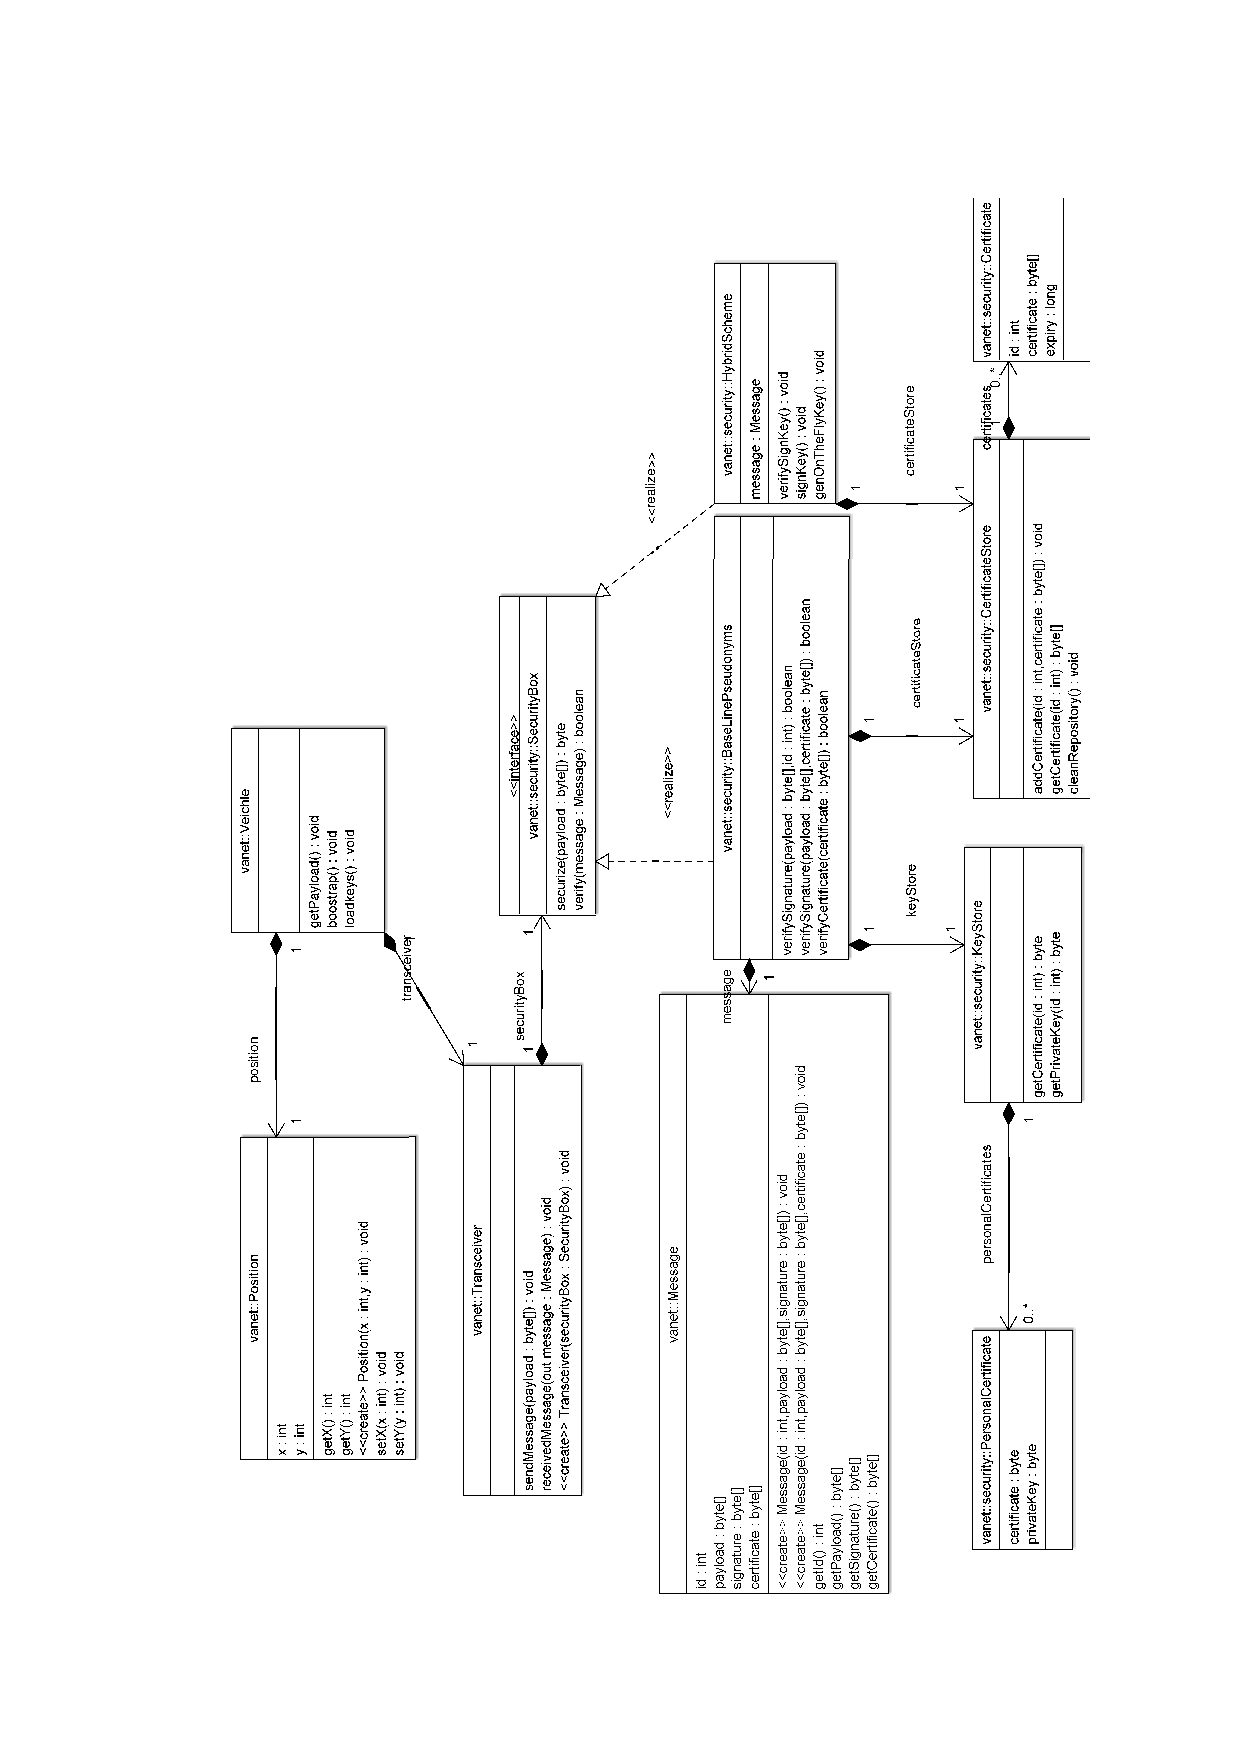
\includegraphics{class_diagram.pdf}}
% otherwise see the example in the following (commented out) line
% to scale it relatively to the page width
\centerline{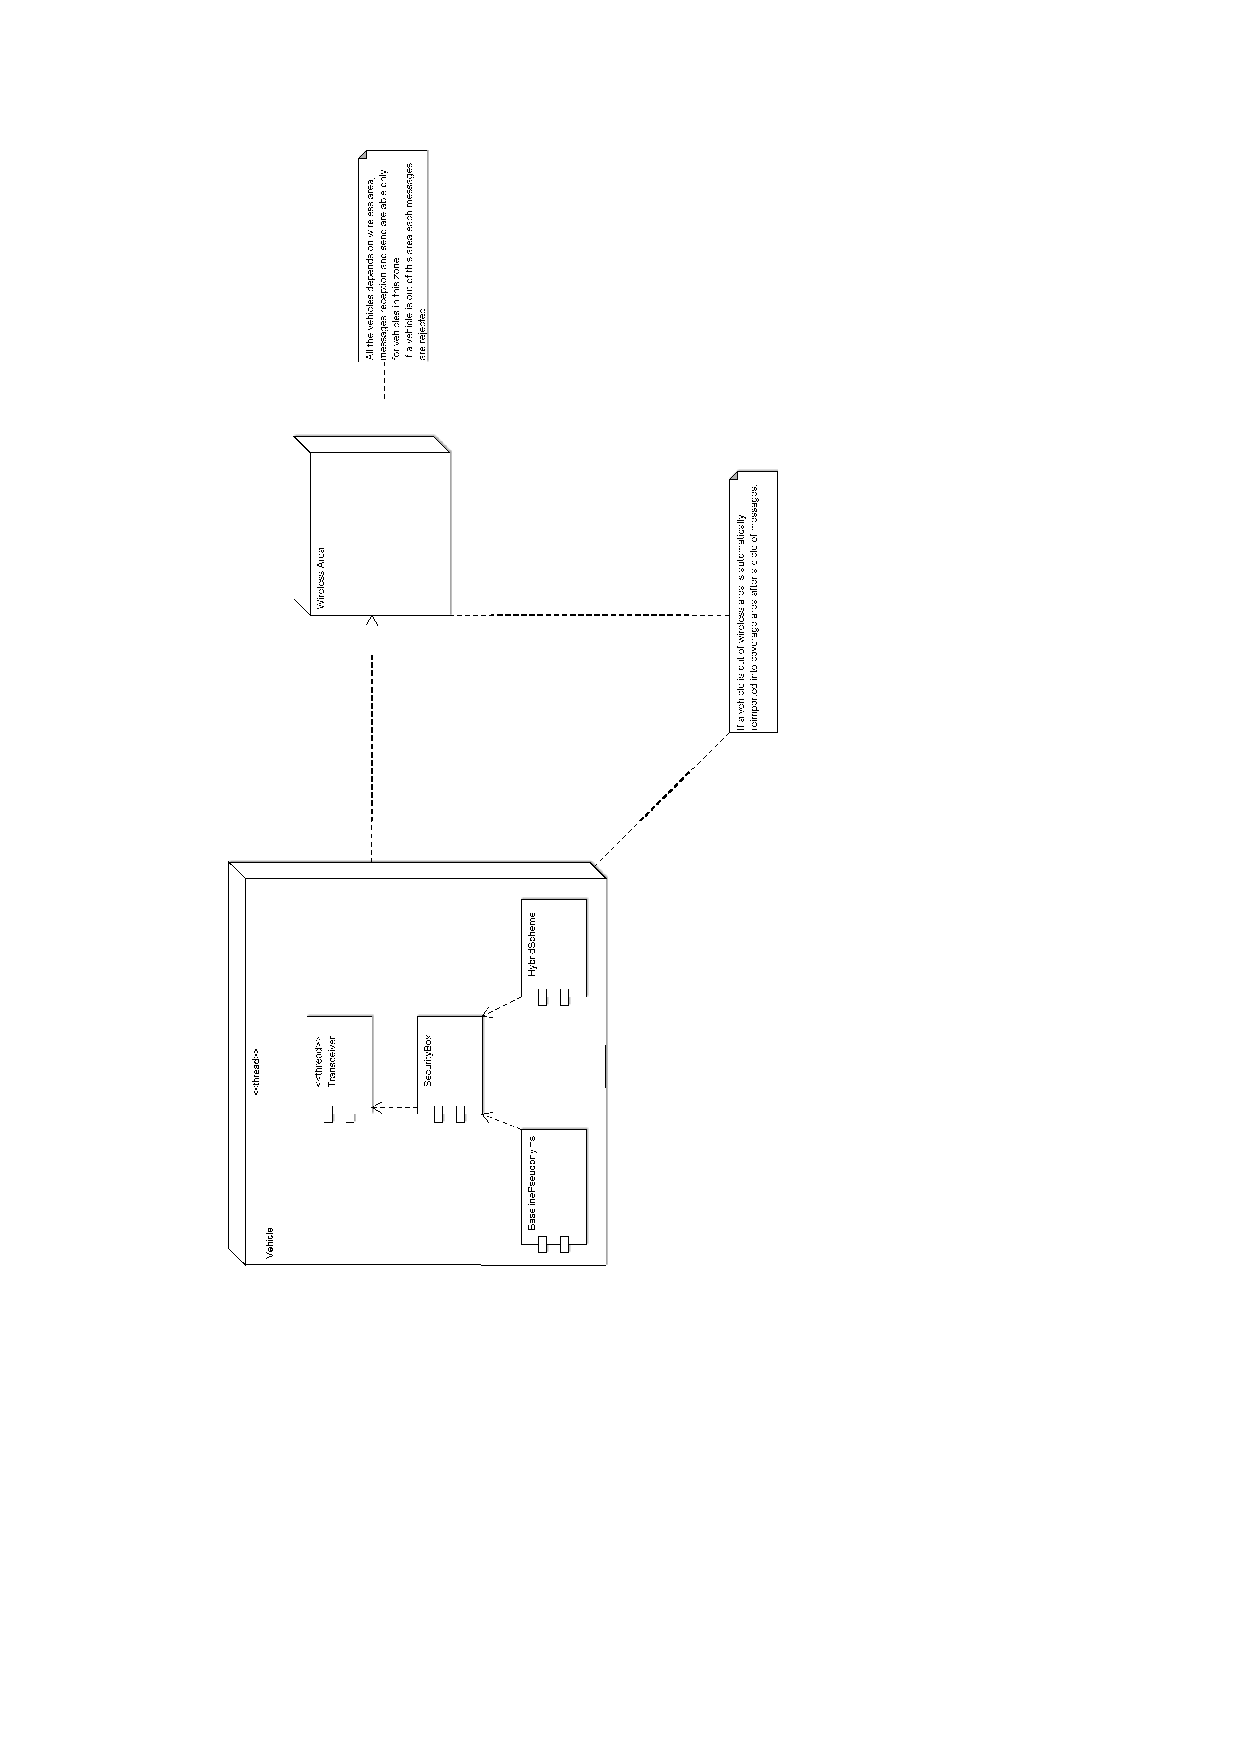
\includegraphics[width=0.6\textwidth, angle=-90]{vanet_stack.pdf}}
\caption{Vanet Stack}
\label{fig:vanet_stack}
\end{figure}

\subsection{Class Diagram}
\begin{figure}[ht]
% If the picture uses fonts of the correct size (10 ... 12 pt)
% then can be included without scaling
%\centerline{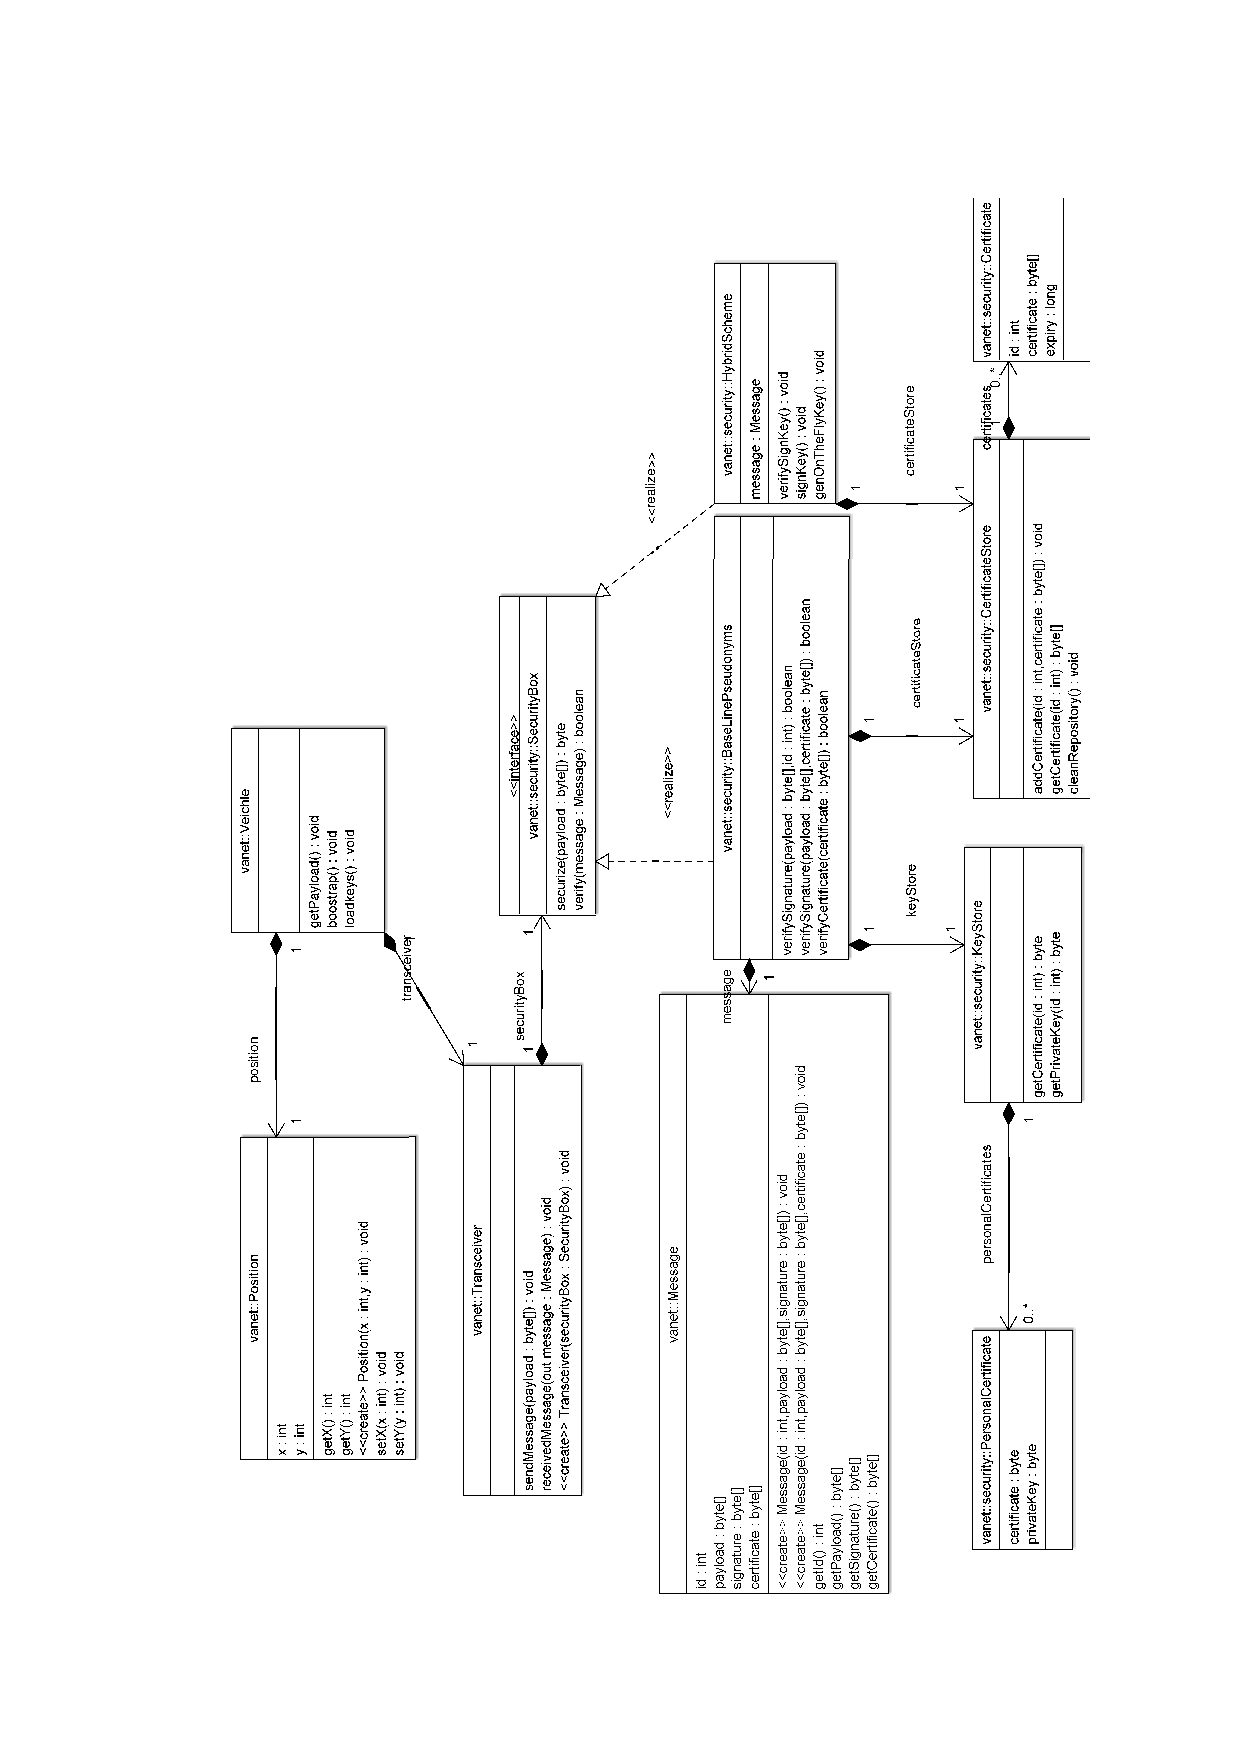
\includegraphics{class_diagram.pdf}}
% otherwise see the example in the following (commented out) line
% to scale it relatively to the page width
\centerline{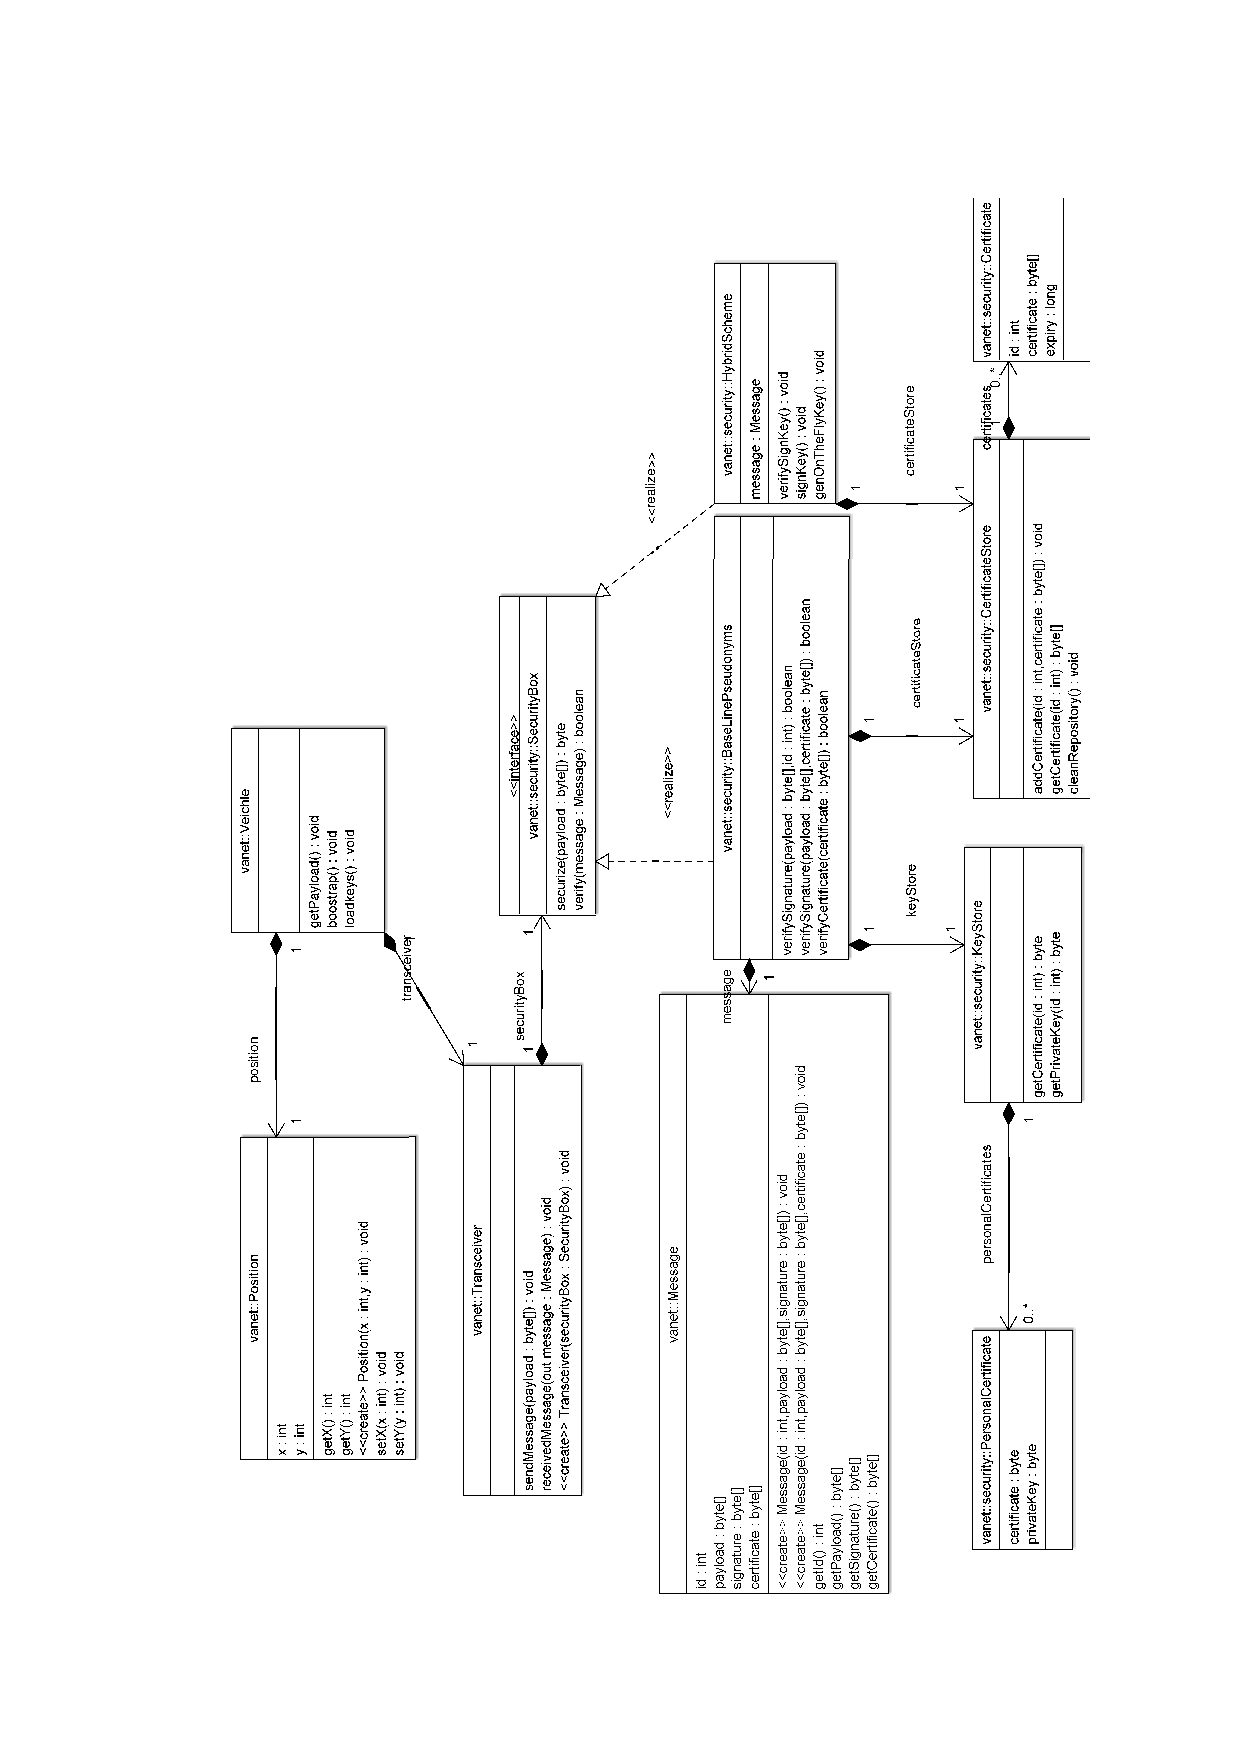
\includegraphics[width=0.9\textwidth]{class_diagram.pdf}}
\caption{Class Diagram}
\label{fig:class_diagram}
\end{figure}